\documentclass{beamer}
%Imports and customization
\usepackage{tikz}
\usepackage{graphicx}
\usepackage{tikz-feynman}
\graphicspath{ 
    {./images/}
}

\beamertemplatenavigationsymbolsempty
\setbeamertemplate{sidebar right}{}
\setbeamertemplate{footline}{
    \hfill\usebeamertemplate***{navigation symbols}
    \hspace{1cm}\insertframenumber{}/\inserttotalframenumber
}
\setbeamertemplate{caption}{\raggedright\insertcaption\par}
\setbeamersize{text margin left=5mm,text margin right=5mm} 

\setbeamerfont{itemize/enumerate body}{size=\scriptsize}
\setbeamerfont{itemize/enumerate subbody}{size=\scriptsize}
\setbeamerfont{itemize/enumerate subsubbody}{size=\scriptsize}


%Custom Macros
\newcommand{\statwarn}{
    \tiny \color{red} Absolute numbers here mean NOTHING. Plots are based on small (100k events) samples, and are highly biased. All that matters is relative position!
}


\newcommand{\fullscreenimage}[2]{
    \frame{
        \frametitle{#1} 
        \begin{figure}
        \includegraphics[height=0.9\textheight,keepaspectratio]{#2}
        \end{figure}
    }
}


\newcommand{\displayone}[3]{
    \frame{
        \frametitle{#1} 
        \begin{columns}
            \begin{column}{0.5\textwidth}
                #2
            \end{column}
            \begin{column}{0.5\textwidth}
                \begin{figure}
                    \includegraphics[width=\linewidth,height=\textheight,keepaspectratio]{#3}
                \end{figure}
            \end{column}
        \end{columns}
    }
}

\newcommand{\displayonelarge}[3]{
    \frame{
        \frametitle{#1} 
        \begin{columns}
            \begin{column}{0.3\textwidth}
                #2
            \end{column}
            \begin{column}{0.7\textwidth}
                \begin{figure}
                    \includegraphics[width=\linewidth,height=\textheight,keepaspectratio]{#3}
                \end{figure}
            \end{column}
        \end{columns}
    }
}


\newcommand{\displaytwo}[4]{
    \frame{
        \frametitle{#1} 
        #2
        \begin{columns}
            \begin{column}{0.5\textwidth}
                \begin{figure}
                    \includegraphics[width=\linewidth,height=\textheight,keepaspectratio]{#3}
                \end{figure}
            \end{column}
            \begin{column}{0.5\textwidth}
                \begin{figure}
                    \includegraphics[width=\linewidth,height=\textheight,keepaspectratio]{#4}
                \end{figure}
            \end{column}
        \end{columns}
    }
}


\newcommand{\displaythree}[5]{
    \frame{
        \begin{columns}[T]
            \begin{column}{0.5\textwidth}
                \insertframetitle{#1}\\
                #2
            \end{column}
            \begin{column}{0.5\textwidth}
                \begin{figure}
                    \includegraphics[width=\linewidth,height=\textheight,keepaspectratio]{#3}
                \end{figure}
            \end{column}
        \end{columns}
        \begin{columns}[T]
            \begin{column}{0.5\textwidth}
                \begin{figure}
                    \includegraphics[width=\linewidth,height=\textheight,keepaspectratio]{#4}
                \end{figure}
            \end{column}
            \begin{column}{0.5\textwidth}
                \begin{figure}
                    \includegraphics[width=\linewidth,height=\textheight,keepaspectratio]{#5}
                \end{figure}
            \end{column}
        \end{columns}
    }
}


\newcommand{\announcesection}[1]{
    \section{#1}
    \frame{
        \begin{center}
            {\huge #1} 
        \end{center}
    }
}


%Begin Presentation
\begin{document}
    \title{ Status Report: Online Monitoring and VBF/ggF Discrimination in Di-Higgs }
    \author{Chris Milke}
    \date{18 May, 2020}

    \frame{\titlepage}
    \frame{\frametitle{Overview} \tableofcontents}

    \section{Online Monitoring Migration}

\displaythree{B-Jet Trigger Online Monitoring}
{ \small The Athena monitoring code is used to monitor the functionality of the ATLAS and the HLT while running }
{old_variables/jet_pt} 
{old_variables/jf_ntrkv} 
{old_variables/tag_MV2c10} 

\frame{
    \frametitle{ Original B-Jet Trigger Online Monitered Variables }
    \begin{center} \resizebox{0.95\textheight}{!}{
        \begin{tabular}{ |l|l|l| }
        \hline
      \textbf {Algorithm} & \textbf {Histograms} & \textbf {Title} \\
        \hline
                         &   sv1\_mass     &  BtagFex SV Mass \\
                         &   sv1\_evtx     &  BtagFex SV Energy Fraction \\
                         &   sv1\_nvtx     &  BtagFex SV Two-Track Vertex Number \\
                         &   tag\_IP2D     &  BtagFex IP2D Likelihood Ratio \\
                         &   tag\_IP3D     &  BtagFex IP3D Likelihood Ratio \\
                         &   tag\_SV1      &  BtagFex SV1 Likelihood Ratio \\
                         &   tag\_IP3DSV1  &  BtagFex IP3D+SV1 Discriminant \\
                         &   tag\_MV2c10   &  BtagFex MV2c10 Discriminant \\
                         &   tag\_MV2c20   &  BtagFex MV2c20 Discriminant \\
  EFBtagFexSplit\_EFID,  &   jet\_pt       &  BtagFex Jet PT \\
  EFBtagFex\_EFID        &   jet\_eta      &  BtagFex Jet Eta \\
                         &   tag\_IP2\_c   &  BtagFex IP2D Likelihood Ratio between b and c-jets \\
                         &   tag\_IP2\_cu  &  BtagFex IP2D Likelihood Ratio between c and light-jets \\
                         &   tag\_IP3\_c   &  BtagFex IP2D Likelihood Ratio between b and c-jets \\
                         &   tag\_IP3\_cu  &  BtagFex IP2D Likelihood Ratio between c and light-jets \\
                         &   sv1\_ntkv     &  BtagFex SV Number of tracks used in the SV \\
                         &   sv1\_Lxy      &  BtagFex SV Transverse distance between PV and SV \\
                         &   sv1\_L3d      &  BtagFex SV Distance between PV and SV \\
                         &   sv1\_sig3     &  BtagFex SV 3D Vertex Significance \\
                         &   sv1\_dR       &  BtagFex SV delta R \\
                         &   jf\_n2tv      &  BtagFex JetFitter Number of 2-track vertex \\
                         &   jf\_ntrkv     &  BtagFex JetFitter Number of tracks from displaced vertices \\
                         &   jf\_nvtx      &  BtagFex JetFitter Number of displaced vertices \\
                         &   jf\_nvtx1t    &  BtagFex JetFitter Number of displaced vertices wih 1-track \\
                         &   jf\_mas       &  BtagFex JetFitter Jet mass \\
                         &   jf\_efrc      &  BtagFex JetFitter Jet efrac \\
                         &   jf\_dR        &  BtagFex JetFitter Delta R \\
                         &   jf\_sig3      &  BtagFex JetFitter 3D vertex significance \\
             \hline
                         &   gsc\_ntrk     &  GSCFex Number of tracks \\
                         &   gsc\_width    &  GSCFex Track width \\
     TrigGSCFex          &   gsc\_ptsm     &  GSCFex Sum of tranverse momentum of tracks \\
                         &   gsc\_ptdiff   &  GSCFex PT difference between uncal jet and cal jets \\
                         &   gsc\_ptratio  &  GSCFex PT ratio \\
            \hline
    \end{tabular}
    } \end{center}
}

\frame{
    \frametitle{Current Set of Variables (Validated!)}
    (Fullsize images in backup...)
    \begin{columns}
        \begin{column}{0.6\textwidth}
            \resizebox{0.8\textheight}{!}{
                \begin{tabular}{ |l|l| }
                    \hline
                    \textbf {Histograms} & \textbf {Title} \\
                    \hline
                    jet\_count    &    BtagFexMT Number of Jets \\
                    track\_count  &    BtagFexMT Number of Tracks \\
                    vertex\_count &    BtagFexMT Number of Vertices \\
                    jet\_pt       &  BtagFexMT Jet PT \\
                    jet\_eta      &  BtagFexMT Jet Eta \\
                    track\_Et     &    BtagFexMT Track Transverse Energy \\
                    track\_eta    &    BtagFexMT Track Eta \\
                    track\_phi    &    BtagFexMT Track Phi \\
                    track\_d0     &    BtagFexMT Track D0 \\
                    track\_d0err  &    BtagFexMT Track D0 Error \\
                    track\_d0sig  &    BtagFexMT Track D0 Significance \\
                    track\_z0     &    BtagFexMT Track Z0 \\
                    track\_z0err  &    BtagFexMT Track Z0 Error \\
                    track\_z0sig  &    BtagFexMT Track Z0 Significance \\
                    \hline
                \end{tabular}
            }
        \end{column}
        \begin{column}{0.4\textwidth}
            \begin{figure}
                \includegraphics[height=0.8\textheight,keepaspectratio]{variables_signed_off}
            \end{figure}
        \end{column}
    \end{columns}
}


\displayonelarge{Latest Merge Request was Successful}
{ \small Most recent merge added no functionality,
    but moved monitoring code to a more appropriate algorithm 
    {\tiny (TrigBjetBtagHypoAlgMT)}.\\ \vspace{7mm}
    More variables and adjusted axes in next merge.  }
{merge_request}

    \section{ Di-Higgs Analysis }
\fullscreenimage{VBF Di-Higgs Analysis}{vbf-hh_diagrams}
\frame{
    \frametitle{ VBF $\rightarrow$ HH $\rightarrow$ \fourB }

    \begin{columns}
        \begin{column}{0.5\textwidth}
            { \small
                Goal is to put a better limit on the $C_{2V}$ coupling constant.
            }

            \begin{figure}
                \includegraphics[width=\linewidth,height=\textheight,keepaspectratio]
                {dihiggs_task_list}
            \end{figure}
        \end{column}
        \begin{column}{0.5\textwidth}
            \resizebox{0.50\textheight}{!}{
                \begin{tikzpicture} \begin{feynman}
    \vertex (c2v) {\tiny $C_{2V}$};
    \vertex [above right=of c2v] (h1) {H};
    \vertex [below right=of c2v] (h2) {H};
    \vertex [above left=of c2v] (vb1);
    \vertex [below left=of c2v] (vb2);
    \vertex [left=of vb1] (q1i) {q};
    \vertex [left=of vb2] (q2i) {q};
    \vertex [above right=of h1] (b1) {$b$};
    \vertex [below right=of h2] (bbar2) {$\bar b$};
    \vertex [below=of b1] (bbar1) {$\bar b$};
    \vertex [above=of bbar2] (b2) {$b$};

    \vertex [above=of b1] (q1f) {q};
    \vertex [below=of bbar2] (q2f) {q};

    \diagram* {
        (q1i) -- (vb1) -- (q1f),
        (q2i) -- (vb2) -- (q2f), 
        (vb1) -- [boson] (c2v) -- [boson] (vb2),
        (h1) -- [scalar] (c2v) -- [scalar] (h2),
        (b1) -- (h1) -- (bbar1),
        (b2) -- (h2) -- (bbar2),
    };
\end{feynman} \end{tikzpicture}

            }
        \end{column}
    \end{columns}
}

\section{Analysis Baseline Status}

\displayonelarge{VBF Selection Process Overview}{
    Selection of VBF events from data is done through a series of selection "filters"
}{cutflows/general}

\displayonelarge{VBF-Specific Selections}{
    {\tiny \begin{itemize}
        \item VBF Pair: Remove events in which there are fewer than two jets that are {\bf not} btagged
        \item VBF dEta: Select the jet pair with the highest invariant mass as the  "VBF Pair".\\Remove events where the $\Delta \eta$ of this pair is less than 3
        \item VBF mjj: Remove events where the "VBF Pair's" invariant mass is less than 1000 GeV
    \end{itemize} }
}{cutflows/vbf_only}

\displaytwo{ggF vs VBF for Various \cvv Values}{
    Current selection process across ggF and varying values of \cvv
}{cutflows/c2v_compare}{cutflows/c2v_compare_log}

\fullscreenimage{ROC Curves!}{roc_explanation}
\fullscreenimage{Comparing Selection Performance}{roc_explanation}
\fullscreenimage{Current Selection Method Performance}{rocs/rocs_initial}

\displayonelarge{Baseline BDT}{
    As a baseline, train BDT with same inputs as current algorithm. It should perform at least as well.
}{rocs/rocs_bdt1}

\fullscreenimage{Adding Fox-Wolfram Moments to BDT}{fwMoment_ordering}
\displayfour{Fox-Wolfram Distributions}
{fw_moments/fox-wolfram_1}
{fw_moments/fox-wolfram_2}
{fw_moments/fox-wolfram_3}
{fw_moments/fox-wolfram_4}


\displaytwo{BDT with Fox-Wolfram Moments}{
    Improvent from first seven FW Moments is minor, but noticeable.
}{rocs/rocs_bdt2}{rocs/rocs_bdt2_zoom}


\frame{
    \frametitle{Exploring Multi-Jet Discriminants: Centrality}
    \begin{columns}
        \begin{column}{0.5\textwidth}
            {\small The VBF initial scatter quark jets are not always the only thing present in VBF events.
            Radiated Jets (ISR \& FSR) are not uncommon, and provide additional handles for analysis.}
            \begin{figure}
                \includegraphics[width=\linewidth,height=\textheight,keepaspectratio]{ event_display}
            \end{figure}
        \end{column}
        \begin{column}{0.5\textwidth}
            \begin{center}\resizebox{0.40\textheight}{!}{ 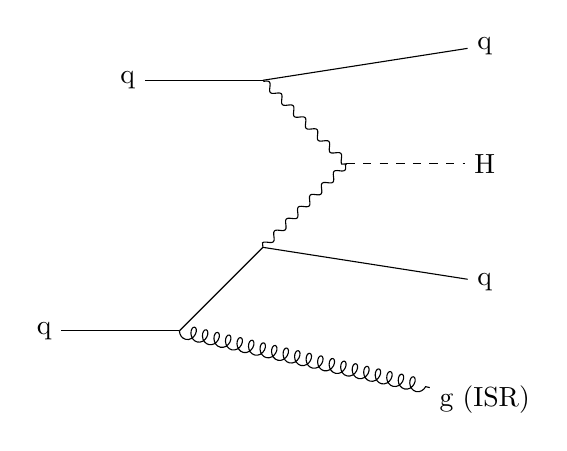
\begin{tikzpicture} \begin{feynman}
    \vertex (a);
    \vertex [right=of a] (b) {H};
    \vertex [above left=of a] (vb1);
    \vertex [below left=of a] (vb2);
    \vertex [left=of vb1] (q1i) {q};
    \vertex [below left=of vb2] (q2k);
    \vertex [left=of q2k] (q2i) {q};
    \vertex [above =of b] (q1f) {q};
    \vertex [below =of b] (q2f) {q};
    \vertex [below =of q2f] (g) {g (ISR)};

    \diagram* {
        (q1i) -- (vb1) -- (q1f),
        (q2i) -- (q2k) -- (vb2) -- (q2f),
        (q2k) --[gluon] (g),
        (vb1) -- [boson] (a) -- [boson] (vb2),
        (a) -- [scalar] (b),
    };
\end{feynman} \end{tikzpicture}
 }\end{center}
            \begin{center}\resizebox{0.40\textheight}{!}{ \begin{tikzpicture} \begin{feynman}
    \vertex (a);
    \vertex [right=of a] (b) {H};
    \vertex [above left=of a] (vb1);
    \vertex [below left=of a] (vb2);
    \vertex [left=of vb1] (q1i) {q};
    \vertex [left=of vb2] (q2i) {q};
    \vertex [below right=of vb2] (q2k);
    \vertex [above =of b] (q1f) {q};
    \vertex [below =of b] (q2f) {q};
    \vertex [below =of q2f] (g) {g (FSR)};

    \diagram* {
        (q1i) -- (vb1) -- (q1f),
        (q2i) -- (vb2) -- (q2k) -- (q2f), 
        (q2k) --[gluon] (g),
        (vb1) -- [boson] (a) -- [boson] (vb2),
        (a) -- [scalar] (b),
    };
\end{feynman} \end{tikzpicture}
 }\end{center}
        \end{column}
    \end{columns}
}


\fullscreenimage{Centrality Distribution}{centrality}
\displaytwo{Centrality as a BDT Input}{
    Improvement from Centrality is very small,
    but there may be more to be gained with further study.
}{rocs/rocs_centrality}{rocs/rocs_centrality_zoom0}


    % Roc curve time! Use mjj distro and cumalitive distro to explain how I made roc curves
    % Now show the unweighted roc curves to show the different performances
    % Show my BDT
    % Now dissapoint everyone with the weighted version... hey steve, how do I weight stuff in SKlearn BDTs?

    % Oh, I should probably mention how my DOE contract is ending so I'm wrapping things up and will soon be back in Dallas

    \section{Conclusion}
    \frame{
        \frametitle{Conclusions}
        \begin{itemize} {
            \item The migration of B-Jet Trigger Monitoring Variables is still moving along well
            \item I've joined the 4b di-Higgs group to assist with VBF jet selection
            \item I have a functional BDT, but it needs lots of work
            \item See y'all back in Dallas soon*
        } \end{itemize}
    }

    \announcesection{Backup}
    \foreach \plot in {jet_count, jet_eta, jet_pt,
    track_count, track_d0err, track_d0sig,
    track_d0, track_eta, track_Et,
    track_phi, track_phi_vs_track_eta, track_z0err,
    track_z0, track_z0sig, vertex_count}
{ \fullscreenimage{}{new_variables/\plot} }

\end{document}
